\section{Electrical Design}
This section describes the electrical layout and components of the fixed and variable pitch quadcopters.

\subsection{Schematic}
In Fig. \ref{fig:fpqsch} the schematic for the FPQ is displayed. This diagram is designed based on the DJI E600 motors. 
\begin{figure}[H]
    \centering
    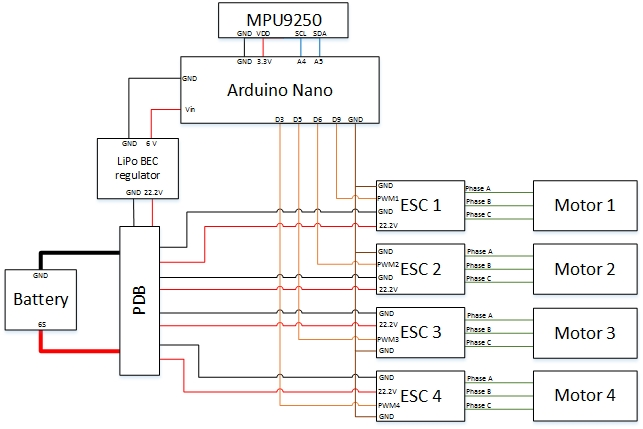
\includegraphics[width = 1\textwidth]{VAPIQ-PICTURES/ShematicFPQ}
    \caption{Schematic for FPQ}
    \label{fig:fpqsch}
\end{figure}
\newpage
\noindent
In Fig. \ref{fig:vpqsch} the schematic for the FPQ is displayed. This diagram is designed based on the AXI 2208/26 motors. 
\begin{figure}[H]
    \centering
    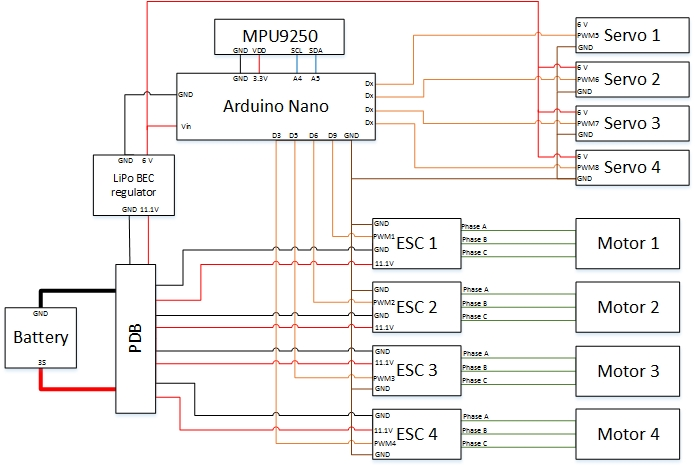
\includegraphics[width = 1\textwidth]{VAPIQ-PICTURES/ShematicVPQ}
    \caption{Schematic for VPQ}
    \label{fig:vpqsch}
\end{figure}
\newpage
\subsection{Components}
In Tab. \ref{tab:CompFPQ} the electrical components needed to construct the FPQ are displayed. This table is designed based on the DJI E600 motors. 
\begin{table}[H]
    \begin{center}
    \caption{Components used for FPQ} 
    \label{tab:CompFPQ} 
        \begin{tabular}{|l|l|c|}
            \hline 
            \textbf{Component:} & \textbf{Info:} & \textbf{Qty.:}  \\ 
            \hline
            Motor & DJI E600  & 4 \\
            ESC & E600 20A & 4 \\
            Bluetooth Module & HC-06 & 1  \\
            Microcontroller & Arduino Nano  ATmega328P& 1 \\
            LiPo Battery & Gens ace 4600mAh, 6S, 35C & 1 \\
            LiPo BEC Regulator & In: 6v-25v, Out: 6V (Max. 5A)  & 1\\
            IMU & MPU9250 & 1 \\
            \hline
        \end{tabular}
    \end{center}
\end{table}
\noindent
To be able to compute the required thrust at hover, the total mass needs to be calculated. In Tab. \ref{tab:WeightFPQ} the mass budget for FPQ is displayed.
\begin{table}[H]
    \begin{center}
    \caption{Mass budget FPQ} 
    \label{tab:WeightFPQ} 
        \begin{tabular}{|l|c|c|}
            \hline 
            \textbf{Component:} & \textbf{Qty.:} & \textbf{Mass[g]:}  \\ 
            \hline
            Frame + cables & 1 & 611.2\\
            Propellers & 4 & 82.8\\
            DJI E600  & 4 & 360 \\
            E600 20A ESC & 4 & 80 \\
            Bluetooth Module HC-06 & 1 & 2\\
            MPU 9250 & 1 & 2 \\
            Arduino Nano & 1 & 7 \\
            LiPo Battery & 1 & 670 \\
            LiPo BEC Regulator & 1 & 19 \\
            PDB & 1 & 20 \\\hline
            \textbf{Total mass budget:} & & 1856\\
            \hline
        \end{tabular}
    \end{center}
\end{table}
\noindent
In Tab. \ref{tab:CompVPQ} the electrical components of the VPQ is displayed. This table is designed based on the AXI 2208/26 motors. 
\begin{table}[H]
    \begin{center}
    \caption{Components used for VPQ} 
    \label{tab:CompVPQ} 
        \begin{tabular}{|l|l|c|}
            \hline 
            \textbf{Component:} & \textbf{Info:} & \textbf{Qty.:}  \\ 
            \hline
            Motor & AXI 2208/26 Gold Line & 4 \\
            ESC & Turnigy Opto 12A & 4 \\
            Servo & Align DS455M, 2.9kg/0.04s & 4  \\ 
            Radio Receiver & Futaba R3008SB & 1  \\
            Microcontroller & Arduino Nano  ATmega328P& 1 \\
            LiPo Battery & Typhon 2200mAh, 3S, 25C & 1 \\
            LiPo BEC Regulator & In: 6v-25v, Out: 6V (Max. 5A)  & 1\\
            IMU & MPU6050 & 1 \\
            \hline
        \end{tabular}
    \end{center}
\end{table}
\noindent
\clearpage
To identify the thrust required for hover, the total mass needs to be calculated. In Tab. \ref{tab:WeightVPQ} the mass budget for VPQ is displayed.
\begin{table}[H]
    \begin{center}
    \caption{Mass budget VPQ} 
    \label{tab:WeightVPQ} 
        \begin{tabular}{|l|c|c|}
            \hline 
            \textbf{Component:} & \textbf{Qty.:} & \textbf{Mass[g]:}  \\ \hline
            Frame & 1 & 83\\
            Propellers + EVP mechanism & 4 & 60\\
            AXI 2208/26 Gold Line  & 4 & 180 \\
            ESC & 4 & 20\\
            Servo & 4 & 80 \\
            Radio Receiver Futaba R3008SB & 1 & 11\\
            MPU 9250 & 1 & 2 \\
            Arduino Nano & 1 & 7 \\
            LiPo Battery & 1 & 153 \\
            LiPo BEC Regulator & 1 & 19 \\
            Miscellaneous & N/A & 146 \\\hline
            \textbf{Total mass budget:} & & 763 \\
            \hline
        \end{tabular}
    \end{center}
\end{table}
\noindent
As seen from Tab. \ref{tab:CompFPQ} and Tab. \ref{tab:CompVPQ}, the only difference in components needed is the servos for the variable pitch quadcopter. 

%bec?

\subsubsection{Electronic Component Description of VPQ}

\textbf{Arduino Nano}\\
The microcontroller used for the flight controller is the Arduino Nano. It was chosen for its size and acceptable computational power \cite{Arduino}. The specifications are listed in Tab. \ref{tab:nanospecs}.

\begin{table}[H]
    \begin{center}
    \caption{Arduino Nano Specs} 
    \label{tab:nanospecs} 
        \begin{tabular}{|l|l|}
            \hline 
                Microcontroller & ATmega328\\
                Operating Voltage & 5V \\
                SRAM & 2 KB\\
                Clock Speed & 16MHz \\
                Analog I/O Pins & 8\\
                Digital I/O Pins & 22\\
                EEPROM & 1 KB\\
                Input Voltage & 7-12V\\
                Weight & 7g\\
                Size & 18x45 mm\\
            \hline
        \end{tabular}
    \end{center}
\end{table}
\\\\

\textbf{AXI 2208/26 Motors}\\
The motors chosen for the variable pitch quadcopter are three phase motors from AXI with hollow shafts. The specific model is AXI 2208/26 Gold Line EVP. These motors have a KV rating of 1420, Kv is the no-load RPM/V. These motors have a high power output, but are light weight. The total weight of the motors with cables is 45g each. 
\\\\

\textbf{ESC}\\
The electronic speed controllers chosen for the AXI motors are from Turnigy Multistar, with input voltage of two to four cells LiPo battery, constant current of 12A and a weight of 6 grams. 
\\\\

\textbf{Servos}\\
To actuate the pitch mechanism, four Align DS455M Digital Servos are used. These are metal geared digital servos with a power of 2.2kg at 6V and a speed of 0.05s per 60 degrees, also at 6V. Each servo weighs 20 grams. 
\\\\

\textbf{LiPo Battery}\\
The specifications of the battery is provided in Tab. \ref{tab:lipospecs}. The battery is from Typhon. 
\begin{table}[H]
    \begin{center}
    \caption{LiPo Battery Specs} 
    \label{tab:lipospecs} 
        \begin{tabular}{|l|l|}
            \hline 
                Capacity & 2200 mAh \\
                Voltage & 11.1V \\
                Number of cells & 3 \\
                C-Rating & 25 \\
                Weight & 153 grams \\
            \hline
        \end{tabular}
    \end{center}
\end{table}
\\\\

\textbf{IMU}\\

\\\\


\newpage
